\documentclass{beamer}
%\documentclass[handout]{beamer}
\usepackage[latin1]{inputenc}


%%%%%%%%%%%%%
%% THEMES w/o navigaton
%\usetheme{default}
%\usetheme{Madrid}
%\usetheme{Pittsburgh}
\usetheme{Boadilla}

%%%%%%%%%%%%%
%% THEMES w/ tree navigation
%\usetheme{Antibes}

%%%%%%%%%%%%%
%% THEMES w/ TOC sidebar
%\usetheme{Berkeley}

%%%%%%%%%%%%%
%% THEMES w/ miniframe navigation
%\usetheme{Berlin}
%\usetheme{Darmstadt}
%\usetheme{Ilmenau}
%\usetheme{Singapore}
%\usetheme{Frankfurt}

%%%%%%%%%%%%%
%% THEMES w/ section/subsection titles
%\usetheme{Copenhagen}
%\usetheme{Warsaw}


%%%%%%%%%%%%%%%

\usecolortheme{beaver}

\usepackage{tikz}
\usetikzlibrary{arrows}

\DeclareMathOperator*{\argmax}{arg\,max}
\DeclareMathOperator*{\argmin}{arg\,min}
%\DeclareMathOperator*{\Em}{E_w(x=x^{(m)},h)}
\DeclareMathOperator*{\Em}{E_w(x^{(m)},h)}
\DeclareMathOperator*{\E}{E_w(x,h)}
\DeclareMathOperator*{\nw}{\nabla_{w_{ij}}}
\newcommand{\btheta}{\boldsymbol \theta }
\newcommand{\bi}{\begin{itemize}}
\newcommand{\ei}{\end{itemize}}
\newcommand{\be}{\begin{enumerate}}
\newcommand{\ee}{\end{enumerate}}

\makeatletter
\def\blfootnote{\xdef\@thefnmark{}\@footnotetext}
\makeatother

\setbeamertemplate{footline}{\hfill\insertframenumber/\inserttotalframenumber}
%\setbeamertemplate{footline}[page number]



\title[Deep Learning]{Deep Learning \& Neural Networks\\Lecture 4}
\author[K. Duh]{Kevin Duh}
\institute[]{Graduate School of Information Science\\Nara Institute of Science and Technology}
\date{Jan 23, 2014}

\begin{document}

\begin{frame}[plain]
\titlepage
\end{frame}


\AtBeginSubsection[]{
\begin{frame}
\frametitle{Today's Topics}
\tableofcontents[currentsection]
\end{frame}
}


%%%%%%%%%%%%%%%%
\begin{frame}
\end{frame}


%%%%%%%%%%%%%
\begin{frame}
\frametitle{Advanced Topics in Optimization}
\bi
\item Today we'll briefly survey an assortment of exciting new tricks for optimizing deep architectures
\item Although there are \textit{many} exciting new things out of NIPS/ICML every year, I'll pick the four that I think is most helpful for practitioners:
\bi
	\item SGD alternative
	\item Better regularization
	\item Scaling to large data
	\item Hyper-parameter search
\ei 
\ei
\end{frame}


%%%%%%%%%


%SECTION%%%%%%%%%%%%%%%%%%%
\section{Hessian-free optimization \cite{martens10hessianfree}}
%%%%%%%%%%%%%%%%%%%%
\begin{frame}
\frametitle{Today's Topics}
\tableofcontents
\end{frame}

\begin{frame}
\frametitle{Difficulty of optimizing highly non-convex loss functions}
\bi
\item "Pathological curvature" is tough to navigate for SGD
\item 2nd-order (Newton) methods may be needed to avoid underfitting
\ei
\centerline{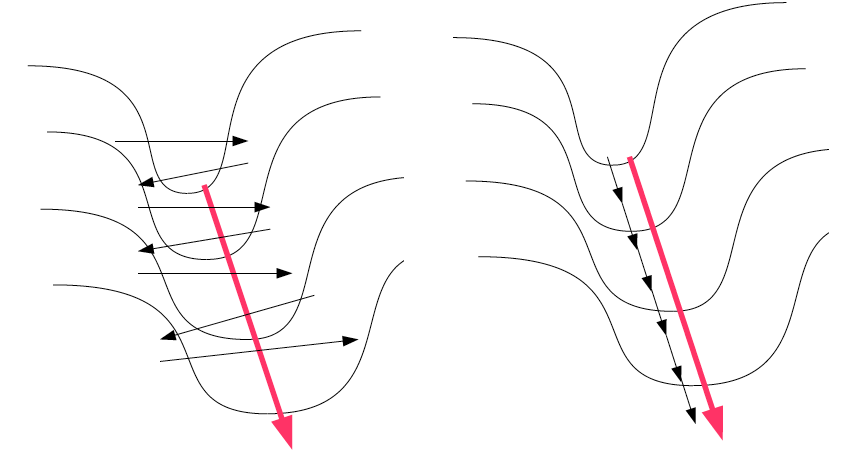
\includegraphics[scale=0.4]{figs/gradient_vs_newton}}
\blfootnote{Figure from \cite{martens10hessianfree}}
\end{frame}

\begin{frame}
\frametitle{2nd-order (Newton) methods}
\bi
\item Idea: approximate the loss function locally with a quadratic\\[0.2cm]
$L(w+z) \approx q_w(z) \equiv L(w) + \nabla L(w)^T z + \frac{1}{2} z^T H z $\\[0.2cm]
\hspace{2cm} where $H$ is the Hessian (curvature matrix) at $w$\\[0.2cm]
\pause
\item Minimizing this gives the search direction: $z^{*}=-H^{-1}\nabla L(w) $
	\bi
	\item Intuitively, $H^{-1}$ fixes any pathological curvature for $\nabla L(w)$
	\item In practice, don't want to store nor invert $H$
	\ei
\pause
\item Quasi-Newton methods
	\bi 
	\item L-BFGS: uses low-rank approximation of $H^{-1}$
	\pause
	\item Hessian-free (i.e. truncated Newton): (1) minimize $q_w(z)$ with conjugate gradient method; (2) computes $Hz$ directly using finite-difference: $Hz = \lim_{\epsilon\rightarrow 0} \frac{\nabla L(w+\epsilon z) - \nabla L(w)}{\epsilon}$
	\ei
\ei
\end{frame}


\begin{frame}
\frametitle{Hessian-free optimization applied to Deep Learning}
\bi
\item \cite{martens10hessianfree} describes some important modifications/settings to make Hessian-free methods work for Deep Learning
\item Experiments:\\[0.2cm]
\begin{center}
(Random initialization + 2nd-order Hessian-free optimizer) \\[0.2cm]
 gives lower training error than \\[0.2cm]
 (Pre-training initialization + 1-order optimizer).\\[0.5cm] 
 \end{center}
 \item Nice results in Recurrent Nets too \cite{martens11recurrent}
\ei
\end{frame}


%SECTION%%%%%%%%%%%%%%%%%%%
\section{Dropout regularization \cite{hinton12dropout}}
%%%%%%%%%%%%%%%%%%%%
\begin{frame}
\frametitle{Today's Topics}
\tableofcontents
\end{frame}

%%%%%%%%%%%%%%%%
\begin{frame}
\frametitle{Dropout \cite{hinton12dropout}}
\begin{columns}
\begin{column}{0.5\textwidth}
\bi
\item Each time we present $x^{(m)}$, randomly delete each hidden node with 0.5 probability
\item This is like sampling from $2^{|h|}$ different architectures 
\item At test time, use all nodes but halve the weights
\item Effect: Reduce overfitting by preventing "co-adaptation"; ensemble model averaging
\ei
\end{column}
\begin{column}{0.5\textwidth}
\begin{center}
\begin{tikzpicture}[->,>=stealth',shorten >=1pt,auto,node distance=3cm,
  thick,main node/.style={circle,fill=blue!20,draw,font=\sffamily\Large\bfseries},cross/.style={path picture={ 
  \draw[red]
(path picture bounding box.south east) -- (path picture bounding box.north west) (path picture bounding box.south west) -- (path picture bounding box.north east);
}}]



  \node[main node] (x1) at (0,0) {$x_1$};
  \node[main node] (x2) at (2,0) {$x_2$};
  \node[main node] (x3) at (4,0) {$x_3$};
  \node[main node] (h1) at (0,2) {$h_1$};
  \node[main node] (h2) at (2,2) {$h_2$};
  \node[main node] (h3) at (4,2) {$h_3$};
  \node[main node] (h'1) at (0,4) {$h'_1$};
  \node[main node] (h'2) at (2,4) {$h'_2$};
  \node[main node] (h'3) at (4,4) {$h'_3$};
  \node[main node] (y) at (2,6) {$y$};
   \node [draw,circle,cross,minimum width=1 cm] at (0,2){}; 
   \node [draw,circle,cross,minimum width=1 cm] at (2,4){}; 
   \node [draw,circle,cross,minimum width=1 cm] at (4,4){}; 


  \path[every node/.style={font=\sffamily\small}]
    (x1) edge node {} (h1)
    (x1) edge node {} (h2)
    (x1) edge node {} (h3)
    (x2) edge node {} (h1)
    (x2) edge node {} (h2)
    (x2) edge node {} (h3)
    (x3) edge node {} (h1)
    (x3) edge node {} (h2)
    (x3) edge node {} (h3)
    (h1) edge node {} (h'1)
    (h1) edge node {} (h'2)
    (h1) edge node {} (h'3)
    (h2) edge node {} (h'1)
    (h2) edge node {} (h'2)
    (h2) edge node {} (h'3)
    (h3) edge node {} (h'1)
    (h3) edge node {} (h'2)
    (h3) edge node {} (h'3)
    (h'1) edge node {} (y)
    (h'2) edge node {} (y)
    (h'3) edge node {} (y) ;

\end{tikzpicture}
\end{center}
\end{column}
\end{columns}
\end{frame}


\begin{frame}
\frametitle{Some Results: TIMIT phone recognition}
\centerline{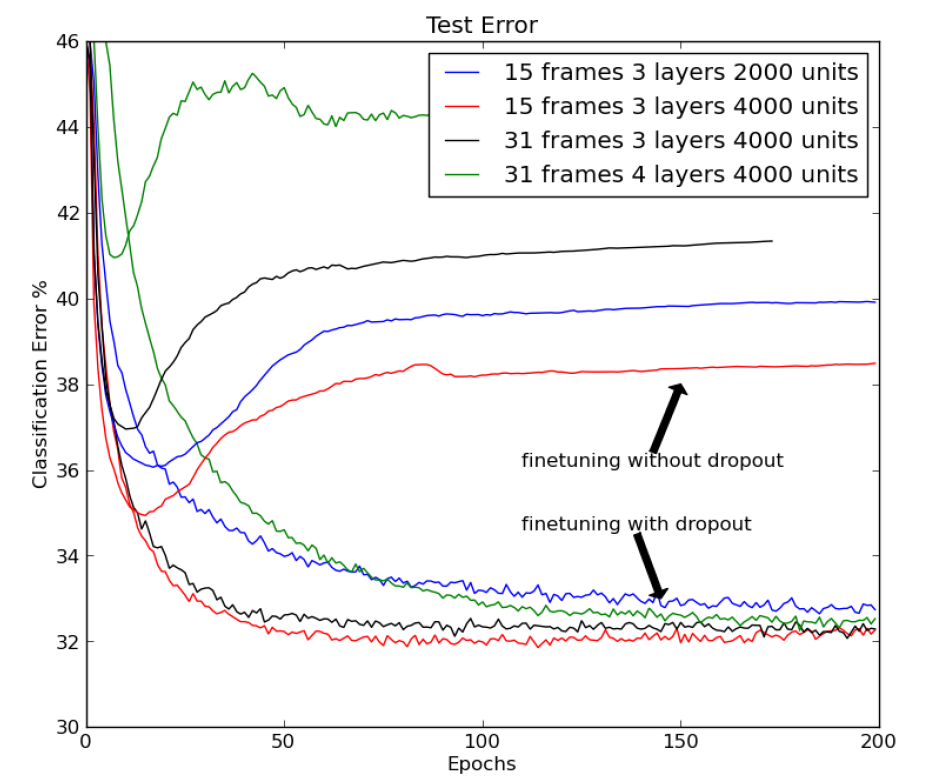
\includegraphics[scale=0.3]{figs/dropout_timit}}
\end{frame}




%SECTION%%%%%%%%%%%%%%%%%%%
\section{Large-scale distributed training \cite{dean12distributed}}
%%%%%%%%%%%%%%%%%%%%
\begin{frame}
\frametitle{Today's Topics}
\tableofcontents
\end{frame}

\begin{frame}
\frametitle{Model Parallelism}
\centerline{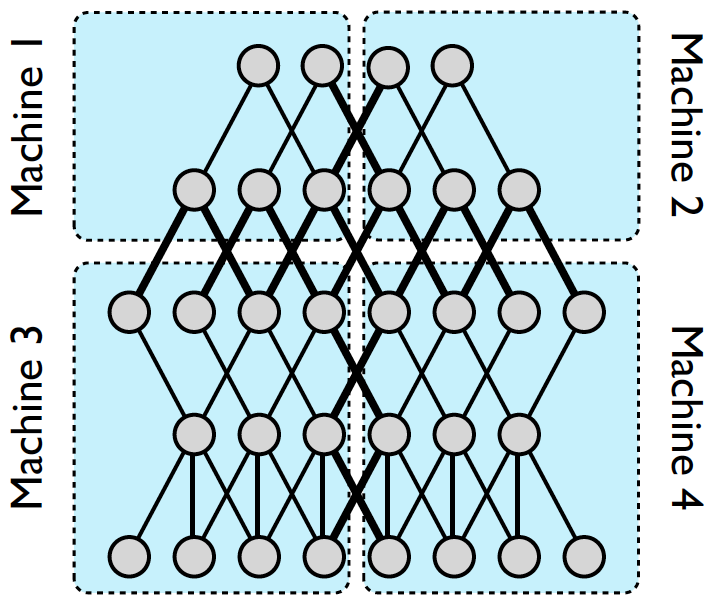
\includegraphics[scale=0.25]{figs/distbelief_model}}
\bi
\item Deep net is stored and processed on multiple cores (multi-thread) or machines (message passing)
\item Performance benefit depends on connectivity structure vs. computational demand
\ei
\blfootnote{Figure from \cite{dean12distributed}}
\end{frame}

\begin{frame}
\frametitle{Data Parallelism}
\centerline{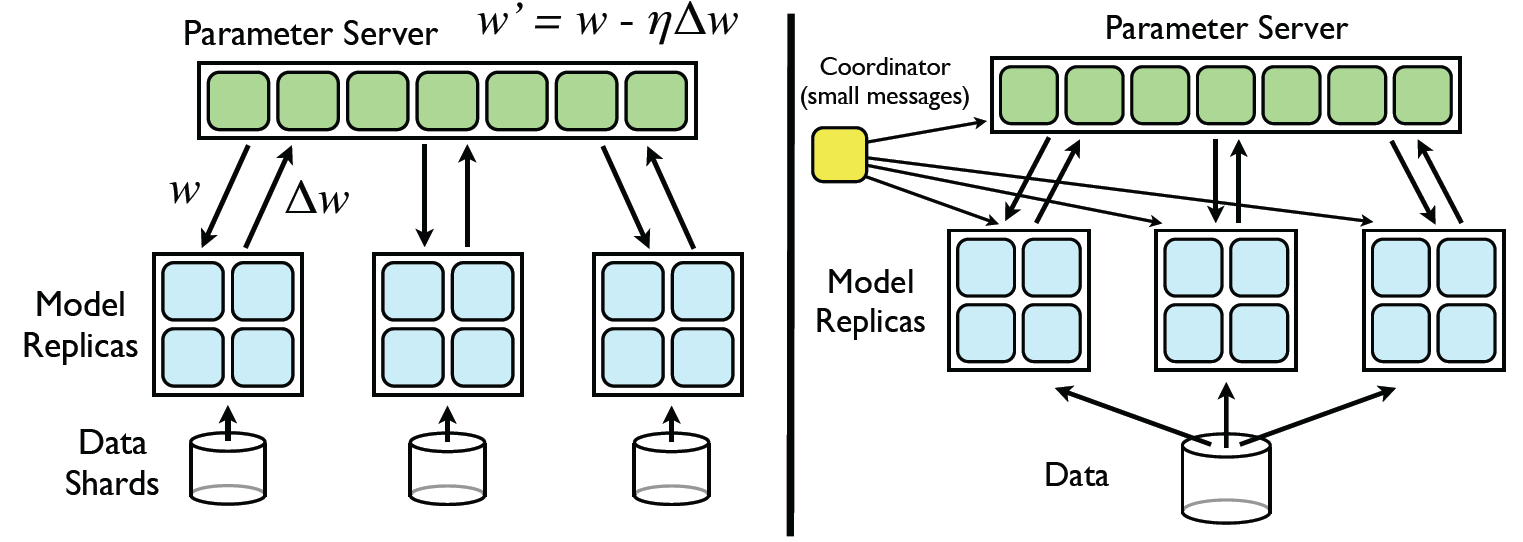
\includegraphics[scale=0.2]{figs/distbelief_data}}
\bi
\item Left: Asynchronous SGD
\bi
	\item Training data is partitioned; different model per shard
	\item Each model pushes and pulls gradient/weight info from parameter server asynchronously$^* \rightarrow$ robust to machine failures
	\item Note gradient updates may be out-of-order and weights may be out-of-date. But it works! (c.f. \cite{langford09slow})
	\item AdaGrad learning rate is beneficial in practice
\ei
\item Right: Distributed L-BFGS 
\ei
\blfootnote{$^*$More precisely, each machine within the model communicates with the relevant parameter server. (Figure from \cite{dean12distributed})}
\end{frame}

\begin{frame}
\frametitle{Performance Analysis}
\centerline{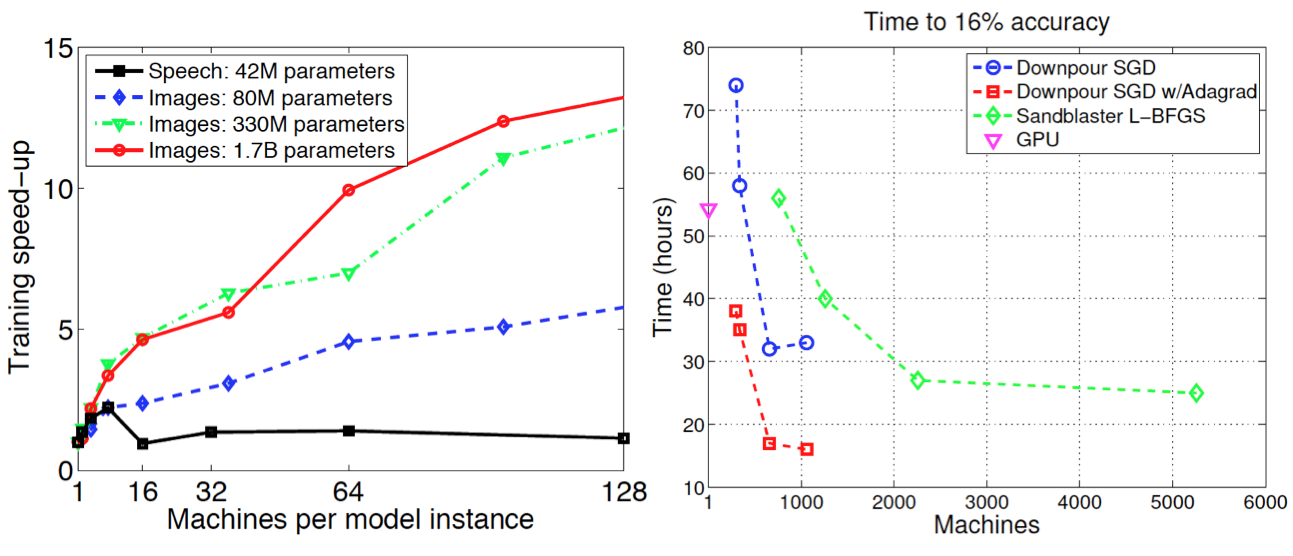
\includegraphics[scale=0.25]{figs/distbelief_result}}
\bi
\item Left: Exploiting model parallelism on a single data shard, up to 12x measured for sparse nets (Images) but diminishing returns. For dense nets (Speech), max at 8 machines.
\item Right: Exploiting data parallelism also, how much time and how many machines are needed to achieve 16\% test accuracy (Speech)? 
\ei
\blfootnote{Figure from \cite{dean12distributed}}
\end{frame}



%SECTION%%%%%%%%%%%%%%%%%%%
\section{Hyper-parameter search \cite{bergstra11hyperparam}}
%%%%%%%%%%%%%%%%%%%%
\begin{frame}
\frametitle{Today's Topics}
\tableofcontents
\end{frame}

\begin{frame}
\frametitle{Hyper-parameter search is important}
\bi
\item Lots of hyper-parameters!
\be
\item Number of layers
\item Number of nodes per layer
\item SGD learning rate
\item Regularization constant
\item Mini-batch size
\item Type of non-linearity
\item Type of distribution for random initialization
\ee
\pause
\vspace{1cm}
\item It's important to invest in finding good settings for your data
\bi
	\item could be the difference between a winning system vs. useless system
\ei
\ei
\end{frame}

\begin{frame}
\frametitle{Approaches to hyper-parameter search}
\be
\item Grid search
\pause
\item Random search
\pause
\item Manual search, a.k.a Graduate Student Descent (GSD)
\pause
\item Treat search itself as a meta machine learning problem \cite{bergstra11hyperparam} 
\bi
	\item Input $x$ = space of hyper-parameters
	\item Output $y$ = validation error after training with given hyper-parameters
\ei
\ee 
\end{frame}

\begin{frame}
\frametitle{Hyper-parameter search as machine learning problem}
\bi
\item Input $x$ = space of hyper-parameters
\item Output $y$ = validation error after training with given hyper-parameters
\ei
\be
\item Computing $y$ is expensive, so we learn a function f(x) that can predict it based on past $(x,y)$ pairs
	\bi
	\item e.g. Linear regression
	\item e.g. Gaussian Process, Parzen Estimator \cite{bergstra11hyperparam}
	\ei
\pause
\item Try the hyper-parameter setting $x^{*} = \arg\min_x f(x)$, or some variant 
\pause
\item Repeat steps 1-2 until you solve AI!
\ee
\end{frame}
	
\begin{frame}[allowframebreaks]
\frametitle{References}
\bibliographystyle{apalike}
\bibliography{mybib}
\end{frame}

\end{document}